\chapter{Agricultura Familiar}
Este cap\'{i}tulo apresenta uma vis\~{a}o geral sobre os trabalhos analisados que possuem tema relacionado ao trabalho sendo apresentado. Dentre os temas relacionados ao trabalho, podemos destacar:

\section{Representação em um Contexto Agrícola}

\subsection{Definição}
A agricultura familiar, cujas diretrizes estão definidas na Lei 11.326 de julho/2006, possui a dinâmica e características bem distintas quando à comparamos com outros tipos de agricultura que não sejam familiares, geralmente seguindo os seguintes requisitos: 

\begin{itemize}
	\item A propriedade objeto da atividade produtiva é compartilhada entre os familiares, utilizando predominantemente a mão-de-obra da própria família.
	\item Utilizam suas terra tanto como local de trabalho, como moradia própria
	\item A direção do estabelecimento deve estár a cargo da prórpia família.
	\item Agricultor não pode possuir área maior que 4 módulos fiscais (valor é diferenciado por município e expresso em hectares) 
\end{itemize}

De acordo com o último censo agropecuário (2006) brasileiro \cite{CENSOAGRO2006}, 84,4\% do total dos estabelecimentos agropecuários brasileiros pertencem a grupos familiares, valor equivalente à aprox. 4,4 milhões de estabelecimentos, constituindo a base econômica de 90\% dos municípios brasileiros com até 20 mil habitantes e 35\% do produto interno bruto nacional, além de possuir grande relevância no abastecimento do mercado interno e controle da inflação dos alimentos.


\begin{figure}[tbh!]
	\centering
	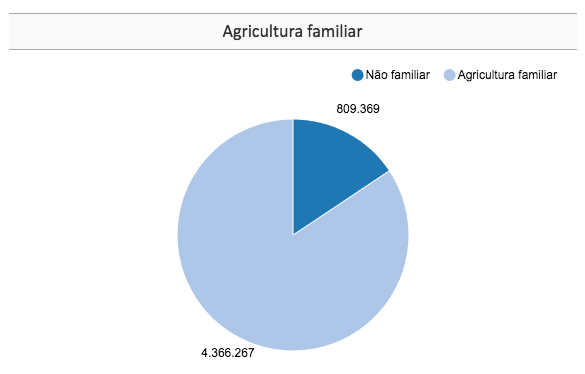
\includegraphics[width=1.0\textwidth]{../images/agriculturaFamiliarTotal}
	\caption{Estabelecimentos agropecuários em relação aos tipos de agricultura}
	\label{fig:agriculturaFamiliarTotal}
\end{figure}

\begin{figure}[tbh!]
	\centering
	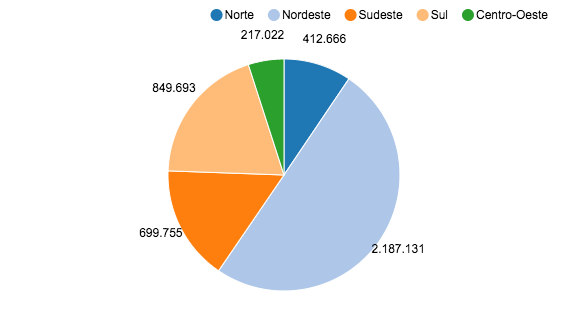
\includegraphics[width=1.0\textwidth]{../images/agriculturaFamiliarRegiao}
	\caption{Estabelecimentos agropecuários familiares em cada regiões administrativa}
	\label{fig:agriculturaFamiliarRegiao}
\end{figure}

\section{Agroecologia}
Agricultura alternativa é um conjunto de práticas e técnicas de cultivo da terra que, diferente da agricultura tradicional, tem como objetivos o desenvolvimento sustentável e a produção de gêneros agrícolas  sem qualquer contaminação por agrotóxicos ou pesticidas. É também conhecida como agricultura ecológica ou agricultura verde.

\subsection{Suas características}

\begin{itemize}
	\item Não utiliza métodos que possam contaminar o solo ou degradá-lo. Os métodos agrícolas utilizados buscam conservar as características e potenciais naturais do solo.
	\item Visa o equilíbrio ecológico na agricultura, respeitando assim o meio ambiente.
	\item Produção de frutas, legumes, grãos e outros gêneros agrícolas sem nenhuma contaminação química. Portanto, os produtos são naturais.
	\item Práticas como queimadas não são empregadas nos processos agrícolas.
	\item Pouca ou nenhuma mecanização.
	\item Uso de mão-de-obra especializada.
	\item Não realiza desmatamentos para geração ou ampliação de áreas agricultáveis.
	\item Áreas de produção próximas às áreas de consumo. Este fator possibilita uso menor de meios de transportes e, por consequência, a redução da poluição do ar.
	\item Uso de fertilizantes naturais.
	\item Uso de métodos naturais de controle de pragas.
	\item Uso racional de recursos naturais (água, por exemplo), evitando assim o desperdício.
	
\end{itemize}


\section{Práticas agrícolas}

Também de acordo com censo agropecuário \cite{CENSOAGRO2006} anteriormente citado, foi feita a análise de identificação dos estabelecimentos segundo a utilização ou não das seguintes práticas agrícolas e seus sub-items: correção da acidez, adubação, controle de pragas e utilização de agrotóxicos.

Considerando o domínio da agricultura familiar, por exemplo, nota-se que fazer o acompanhamento dos níveis de pragas ou agrotóxicos na plantas e acidez, nutrientes e humidade do solo poderia ser facilitado com a utilização de sensores capazes de coletar dados obtidos do meio ambiente utilizado para que sejam processados e analisados por algum sistema de informação, alertando o agricultor quanto aos possíveis riscos encontrados ou tomando decisões utilizando regras préviamente definidas pelo agricultor ou a partir da análise do ciclo de vida do produto. 

Assim, o agricultor precisaria fazer a reposição ou correção do nível de nutrientes, água ou PH apenas quando necessário e nas regiões de plantio que realmente apresentam deficiências, aplicando de forma planejada a estratégia mais adequada para correção do problema encontrado, mantendo o equilíbrio nutricional da planta e proporcionando, assim, um agroecossistema sustentável.


Utilizando métricas encontradas em \cite{}

\begin{figure}[!htb]
	\centering
	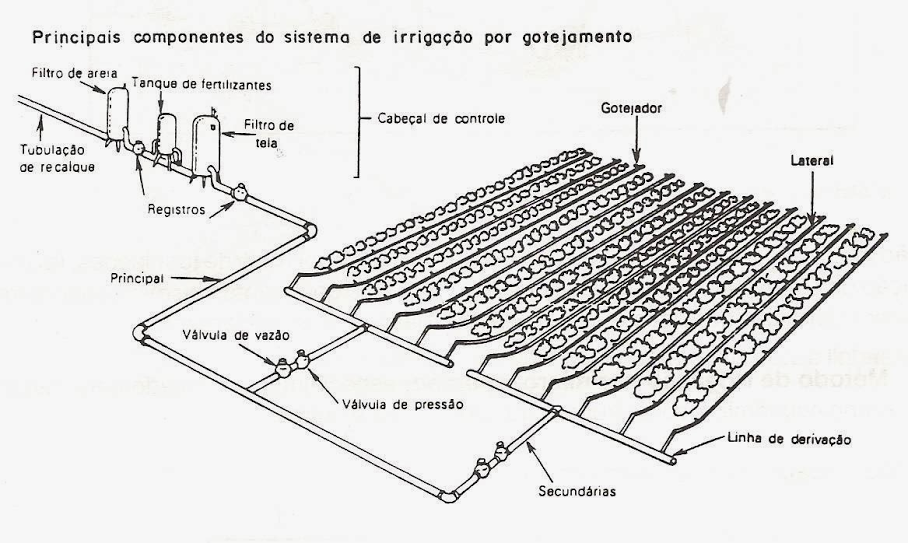
\includegraphics[width=1.0\textwidth]{../images/irrigacao.png}
	\caption{Principais componentes de um sistema de irrigação}
	\label{fig:irrigacao}
\end{figure}

\begin{figure}[!htb]
	\centering
	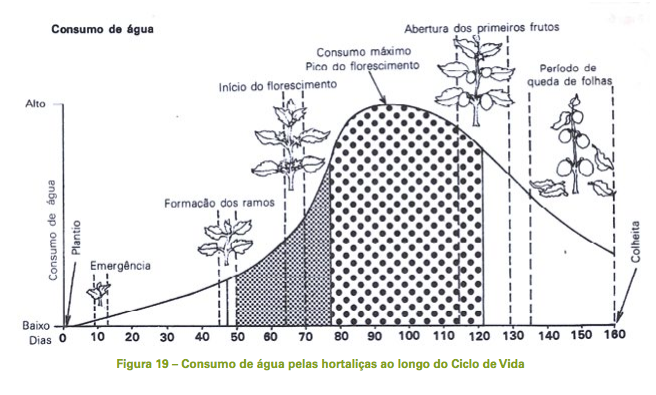
\includegraphics[width=1.0\textwidth]{../images/consumo_de_agua.png}
	\caption{Consumo de água}
	\label{fig:consumoagua}
\end{figure}

\begin{table}[]
	\centering
	\caption{Consumo de \'{a}gua para diferentes hortaliças durante o seu desenvolvimento}
	\label{table:consumo1}
	\begin{tabular}{lc}
		\hline
		Cultura	& Consumo de água/min\(mm\)	\\ 
		\hline
		Batata				& 500 a 800 \\
		Batata-doce			& 400 a 675 \\
		Beterraba			& 100 a 1500 \\
		Cebola				& 350 a 600 \\
		Feijão-de-vagem		& 300 a 500 \\
		Milho-verde			& 400 a 700 \\
		Tomate				& 300 a 600 \\
		Outras hortaliças	& 250 a 500 \\ \hline
	\end{tabular}
\end{table}

\begin{table}[]
	\centering
	\caption{Períodos críticos de deficiência de água para v\'{a}rias hortaliças}
	\label{table:periodocritico}
	\begin{tabular}{ll}
		\hline
		Cultura	& Consumo de água/min\(mm\)\\ 
		\hline
		Alface				& 500 a 800 \\
		Batata-doce			& 400 a 675 \\
		Beterraba			& 100 a 1500 \\
		Cebola				& 350 a 600 \\
		Feijão-de-vagem		& 300 a 500 \\
		Milho-verde			& 400 a 700 \\
		Tomate				& 300 a 600 \\
		Outras hortaliças	& 250 a 500 \\
		\hline
	\end{tabular}
\end{table}

\begin{table}[]
	\centering
	\caption{Tempo (em horas) diário de irrigação por aspersão em função da idade da planta (DAP) e do mês do ano. intervalo de 4 dias entre irrigações.}
	\label{table:consumo2}
	\begin{tabular}{lllllllllllll}
		\hline
		\multicolumn{13}{l}{Milho com uso de microdifusor \(42 l/h\)} \\
		\hline
		DAP	& Jan. & Fev. & Mar. & Abr. & Mai. & Jun. & Jul. & Ago. & Set. & Out. & Nov. & Dez. \\
		Até 25& 0,4& 0,4& 0,4& 0,4& 0,3& 0,3& 0,3& 0,3& 0,5& 0,5& 0,5& 0,4 \\
		26 - 55& 0,7& 0,7& 0,6& 0,6& 0,5& 0,5& 0,5& 0,5& 0,7& 0,8& 0,8& 0,7 \\
		56 - 95& 0,6& 0,6& 0,6& 0,6& 0,5& 0,4& 0,4& 0,5& 0,7& 0,7& 0,7& 0,6 \\
		\hline
		\multicolumn{13}{l}{Melancia com uso de microdifusor \(42 l/h\)} \\ 
		\hline
		DAP & Jan. & Fev. & Mar. & Abr. & Mai. & Jun. & Jul. & Ago. & Set. & Out. & Nov. & Dez. \\			
		Até 25& 0,2& 0,2& 0,2& 0,2& 0,2& 0,2& 0,1& 0,2& 0,2& 0,2& 0,2& 0,2 \\
		25-50& 0,7& 0,7& 0,6& 0,6& 0,5& 0,5& 0,4& 0,5& 0,7& 0,7& 0,7& 0,7 \\
		50-70& 0,4& 0,4& 0,3& 0,3& 0,3& 0,3& 0,2& 0,3& 0,4& 0,4& 0,4& 0,4 \\
		\hline
		\multicolumn{13}{l}{Banana com uso de microdifusor \(42 l/h\)} \\
		\hline
		DAP & Jan. & Fev. & Mar. & Abr. & Mai. & Jun. & Jul. & Ago. & Set. & Out. & Nov. & Dez. \\			
		Até 30& 0,3& 0,3& 0,3& 0,3& 0,2& 0,2& 0,2& 0,2& 0,3& 0,3& 0,3& 0,3 \\
		31 - 210& 0,7& 0,7& 0,6& 0,6& 0,5& 0,5& 0,5& 0,5& 0,7& 0,8& 0,8& 0,7 \\
		211 - 365& 0,6& 0,6& 0,6& 0,6& 0,5& 0,4& 0,4& 0,5& 0,7& 0,7& 0,7& 0,6 \\
		\hline
		\multicolumn{13}{l}{Mam\~{a}o com uso de microdifusor \(42 l/h\)} \\
		\hline
		DAP & Jan. & Fev. & Mar. & Abr. & Mai. & Jun. & Jul. & Ago. & Set. & Out. & Nov. & Dez. \\	
		Até 107& 0,4& 0,4& 0,4& 0,4& 0,3& 0,3& 0,3& 0,3& 0,4& 0,4& 0,4& 0,4 \\
		108 - 260& 0,7& 0,7& 0,7& 0,6& 0,6& 0,5& 0,5& 0,6& 0,8& 0,8& 0,8& 0,7 \\
		261 - 380& 0,7& 0,7& 0,7& 0,7& 0,6& 0,5& 0,5& 0,6& 0,8& 0,8& 0,8& 0,8 \\
		\hline
	\end{tabular}
\end{table}

\subsection{agricultura e tecnologia}

Sensores e atuadores espalhados nas plantações de forma setorizada podem dar informações precisas da  temperatura, umidade, chuva, vento, fertilidade do solo, pragas e outras informações essenciais para a análise do ecossistema. utilizado no plantio.

\begin{figure}[tbh!]
	\centering
	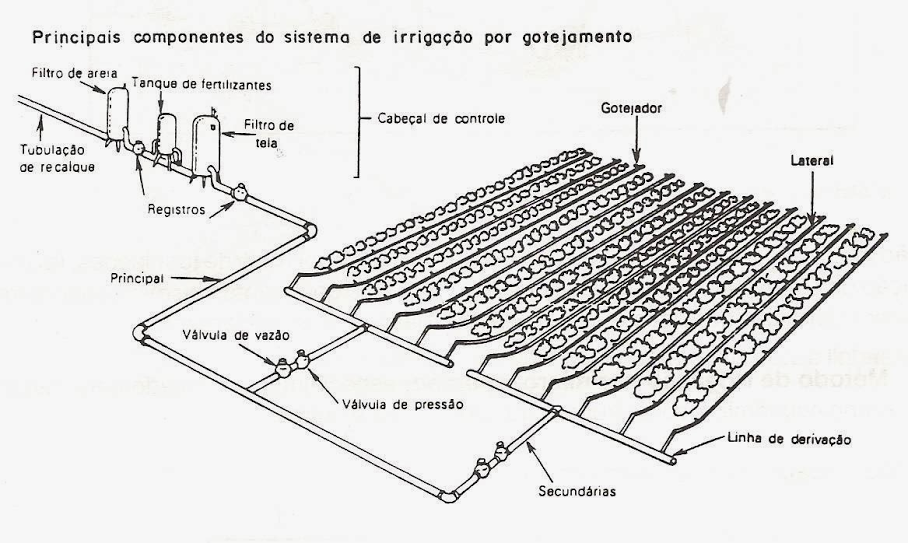
\includegraphics[width=1.0\textwidth]{../images/irrigacao}
	\caption{Sistema de Irrigação por Gotejamento \cite{http://agronegociointerior.com.br/irrigacao-por-gotejamento/ (2016)}
	\label{fig:sistemaGotejamento}
\end{figure}


De igual forma, sensores e atuadores conectados aos reservatórios de água, válvulas de pressão, bomba de água e equipamentos de energia solar e etc. conseguem ajudar no controle de uso dos recursos utilizados;

\begin{figure}[tbh!]
	\centering
	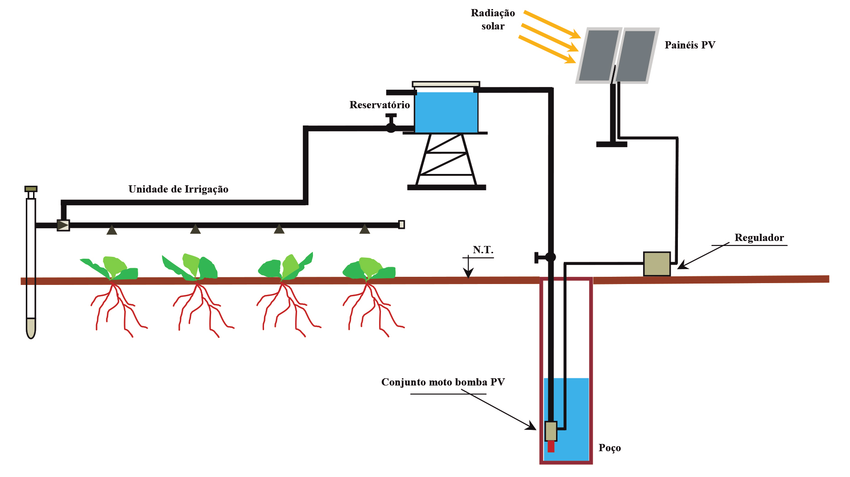
\includegraphics[width=1.0\textwidth]{../images/energia-autonomo}
	\caption{Sistema PV autônomo aplicado à irrigação \cite{Alvarenga,Ferreira,Fortes (2014)} }
	\label{fig:sistemaEnergia}
\end{figure}


\paragraph{Ciclo de vida de produto ou serviço}
 Informações referente a todas as etapas de produção e uso de respectivo produto, desde à extração das matérias-primas necessárias para sua produção, até o seu descarte ou reciclagem, incluíndo seus processos de produção, distribuição, consumo e reuso \cite{IBICT}.  Desde o ano 2000, a organização IBICT é responsável por fomentar o desenvolvimento referente à realidade brasileira, disseminando seus benefícios.


\paragraph{Avaliação do Ciclo de Vida - (ACV)}
%http://acv.ibict.br/acv/o-que-e-o-acv/
%ISO 14040/14044
Metodologia criada para mapear e mensurar possíveis impactos ambientais que a fabricação e uso de um produto ou serviço pode causar ao nosso ecossistema. Inicialmente é feito o processo de lavantamento de todas as informações relevantes ao ciclo de vida dos produtos analisados \cite{IBICT}, buscando uma melhor compreensão do desempenho ambiental de produtos e processos. Enquanto pesquisadores a utilizam para ampliação de sua base científica de conhecimento sobre sistemas produtivo, a indústria se encarrega de utiliza-la para melhoria e eficiência de seus processos, redução dos custos e marketing de seus produtos. Suas fases são


\begin{labeling}[Definição dos Objetivos e Escopo\quad]
\item[Definição dos Objetivos e Escopo] Determinar fronteiras de estudo (temporal e geográfica) do ciclo de vida do produto cultivado, identificando processos que mais impactam o meio ambiente. 
\item[Análise do inventário] Coleta dos dados que representam fluxos de entrada e saída de massa e energia nas diversas etapas do ciclo de vida do produto.
\item[Avaliação de impacto] Análise e calculo dos impactos ambientais a partir dos fluxos definidos no inventário.
\item[Interpretação] identificar questões significativas, checar a integridade, a sensibilidade e a consistência dos resultados.
\end{labeling}
